\documentclass[../main-report.tex]{subfiles}
\begin{document}
\section{Một số lý thuyết về xác suất}
% Tham khảo: https://viblo.asia/p/ly-thuyet-xac-suat-co-ban-su-dung-trong-machine-learning-naQZR78Plvx
Có thể nói một điều rằng lý thuyết xác suất là một trong những lý thuyết quan trọng nhất của khoa học hiện đại và đặc biệt là \textbf{Machine Learning} bởi vì đa phần các thuật toán của Machine Learning đều có cơ sở dựa trên xác suất.
\subsection{Không gian xác suất}
Khi nói đến xác suất là người ta nói đến các lý thuyết toán học về sự \textit{bất định - uncertainly} hay nói một cách khác, xác suất biểu thị khả năng xảy ra của các \textit{sự kiện - event} trong một môi trường bất định nào đó. Ví dụ chúng ta xét về xác suất có mưa hay không có mưa vào thứ hai tuần tới, xác suất tỏ tình thành công hay thất bại của cậu bạn thân,\ldots Tóm lại cứ nói đến xác suất là đề cập đến sự không chắc chắn hay bất định đó.

Về mặt toán học, người ta kí hiệu một \textbf{không gian xác suất - probability space} bao gồm 3 thành phần $(\Omega, F, P)$ như sau:

\begin{itemize}
\item $\Omega$ (có thể đọc là ``Ô-me-ga'') chính là tập các giá trị \textbf{có thể xảy ra - possible outcome} với sự kiện trong không gian xác suất. Người ta còn gọi nó là \textbf{không gian mẫu}.
\item $F \subseteq 2^{\Omega}$ là tập hợp các sự kiện có thể xảy ra trong không gian xác suất.
\item $P$ là xác suất (hoặc phân phối xác suất) của sự kiện. $P$ ánh xạ một sự kiện $E \in F$ vào trong một giá trị thực $p \in \left [ 0;1 \right ]$. Ở đây chúng ta gọi $p = P(E)$ là xác suất của sự kiện $E$.
\end{itemize}

\subsubsection*{Ví dụ minh họa}
Chúng ta cùng nhau xem xét một ví dụ khá kinh điển trong lý thuyết xác suất đó chính là ví dụ \textbf{tung xúc sắc}.

Giả sử rằng chúng ta tung một con xúc sắc 6 mặt. Không gian các \textbf{outcomes} có thể xảy ra trong trường hợp này là $\Omega = \left \{ 1, 2, 3, 4, 5, 6 \right \}$ - chúng ta không tính đến các trường hợp xúc sắc rơi lơ lửng tức là không thuộc mặt nào. Không gian các sự kiện $F$ sẽ tùy thuộc vào sự định nghĩa của chúng ta. Ví dụ chúng ta định nghĩa sự kiện xúc sắc là mặt chẵn hoặc mặt lẻ thì không gian sự kiện $F=\left \{ \varnothing , \left \{ 1, 3, 5 \right \}, \left \{ 2, 4, 6 \right \}, \Omega \right \}$ trong đó $\varnothing$ là sự kiện có xác suất 0 - hay còn gọi là biến cố \textit{không thể có}. $\Omega$ là sự kiện có xác suất 1 - hay còn gọi là \textit{biến cố chắc chắn}.
\subsection{Các tính chất xác suất}
Giống như ví dụ ở phía trên, khi \textit{không gian mẫu - outcomes space} là hữu hạn thì chúng ta thường lựa chọn không gian sự kiện $F=2^{\Omega} = \left \{ \varnothing , \left \{ 1, 3, 5 \right \}, \left \{ 2, 4, 6 \right \}, \Omega \right \}$. Cách tiếp cận này chưa hẳn đã tổng quát hóa cho mọi trường hợp tuy nhiên nó đủ dùng trong các bài toán thực tế, tất nhiên là với giả thiết không gian mẫu của chúng ta là \textbf{hữu hạn}. Khi không gian mẫu là\textbf{ vô hạn - infinite} chúng ta phải hết sức cẩn thận trong việc lựa chọn không gian sự kiện $F$. Khi đã định nghĩa được không gian sự kiện $F$ thì hàm xác suất của chúng ta bắt buộc phải thỏa mãn các tính chất sau đây:

\begin{itemize}
\item \textbf{Không âm - non-negativity} - xác suất của mọi sự kiện là không âm, tức là với mọi $x \in F,~~ P(x)\geq 0$
\item \textbf{Xác suất toàn cục - trivial event} $P(\Omega) = 1$
\item \textbf{Tính cộng - additivity} tức là với mọi $x, y \in F$ nếu như $x\cap y= \varnothing$ thì ta có $P(x\cup y) = P(x) + P(y)$
\end{itemize}
\subsection{Biến ngẫu nghiên}
\textbf{Biến ngẫu nghiên (Random Variables)} là một thành phần quan trọng trong lý thuyết xác suất. Nó biểu diễn giá trị của các đại lượng không xác định, thông thường nó được coi như một ánh xạ từ tập các \textbf{outcomes} trong không gian mẫu thành các giá trị thực.


\subsection{Xác suất có điều kiện}

\subsection{Quy tắc Bayes}

\subsection{Kỳ vọng}

\subsection{Một vài phân phối xác suất thường gặp}

\section{Giới thiệu máy học}
\subsection{Khái niệm}

\subsection{Phân loại}

\section{Thuật toán Decision Tree}
\subsection{Giới thiệu}
Sắp đến kỳ thi, một cậu sinh viên tự đặt ra quy tắc \textit{học hay chơi} của mình như sau:

\begin{itemize}
\item Nếu còn nhiều hơn hai ngày tới ngày thi, cậu sẽ đi chơi.
\item Nếu còn không quá hai ngày và đêm hôm đó có một trận bóng đá, cậu sẽ sang nhà bạn chơi và cùng xem bóng đêm đó.
\item Cậu sẽ chỉ học trong các trường hợp còn lại.
\end{itemize}

Việc ra quyết định của cậu sinh viên này có thể được mô tả trên sơ đồ trong hình \ref{fig:dt_ex1}.

\begin{figure}[ht!]
\centering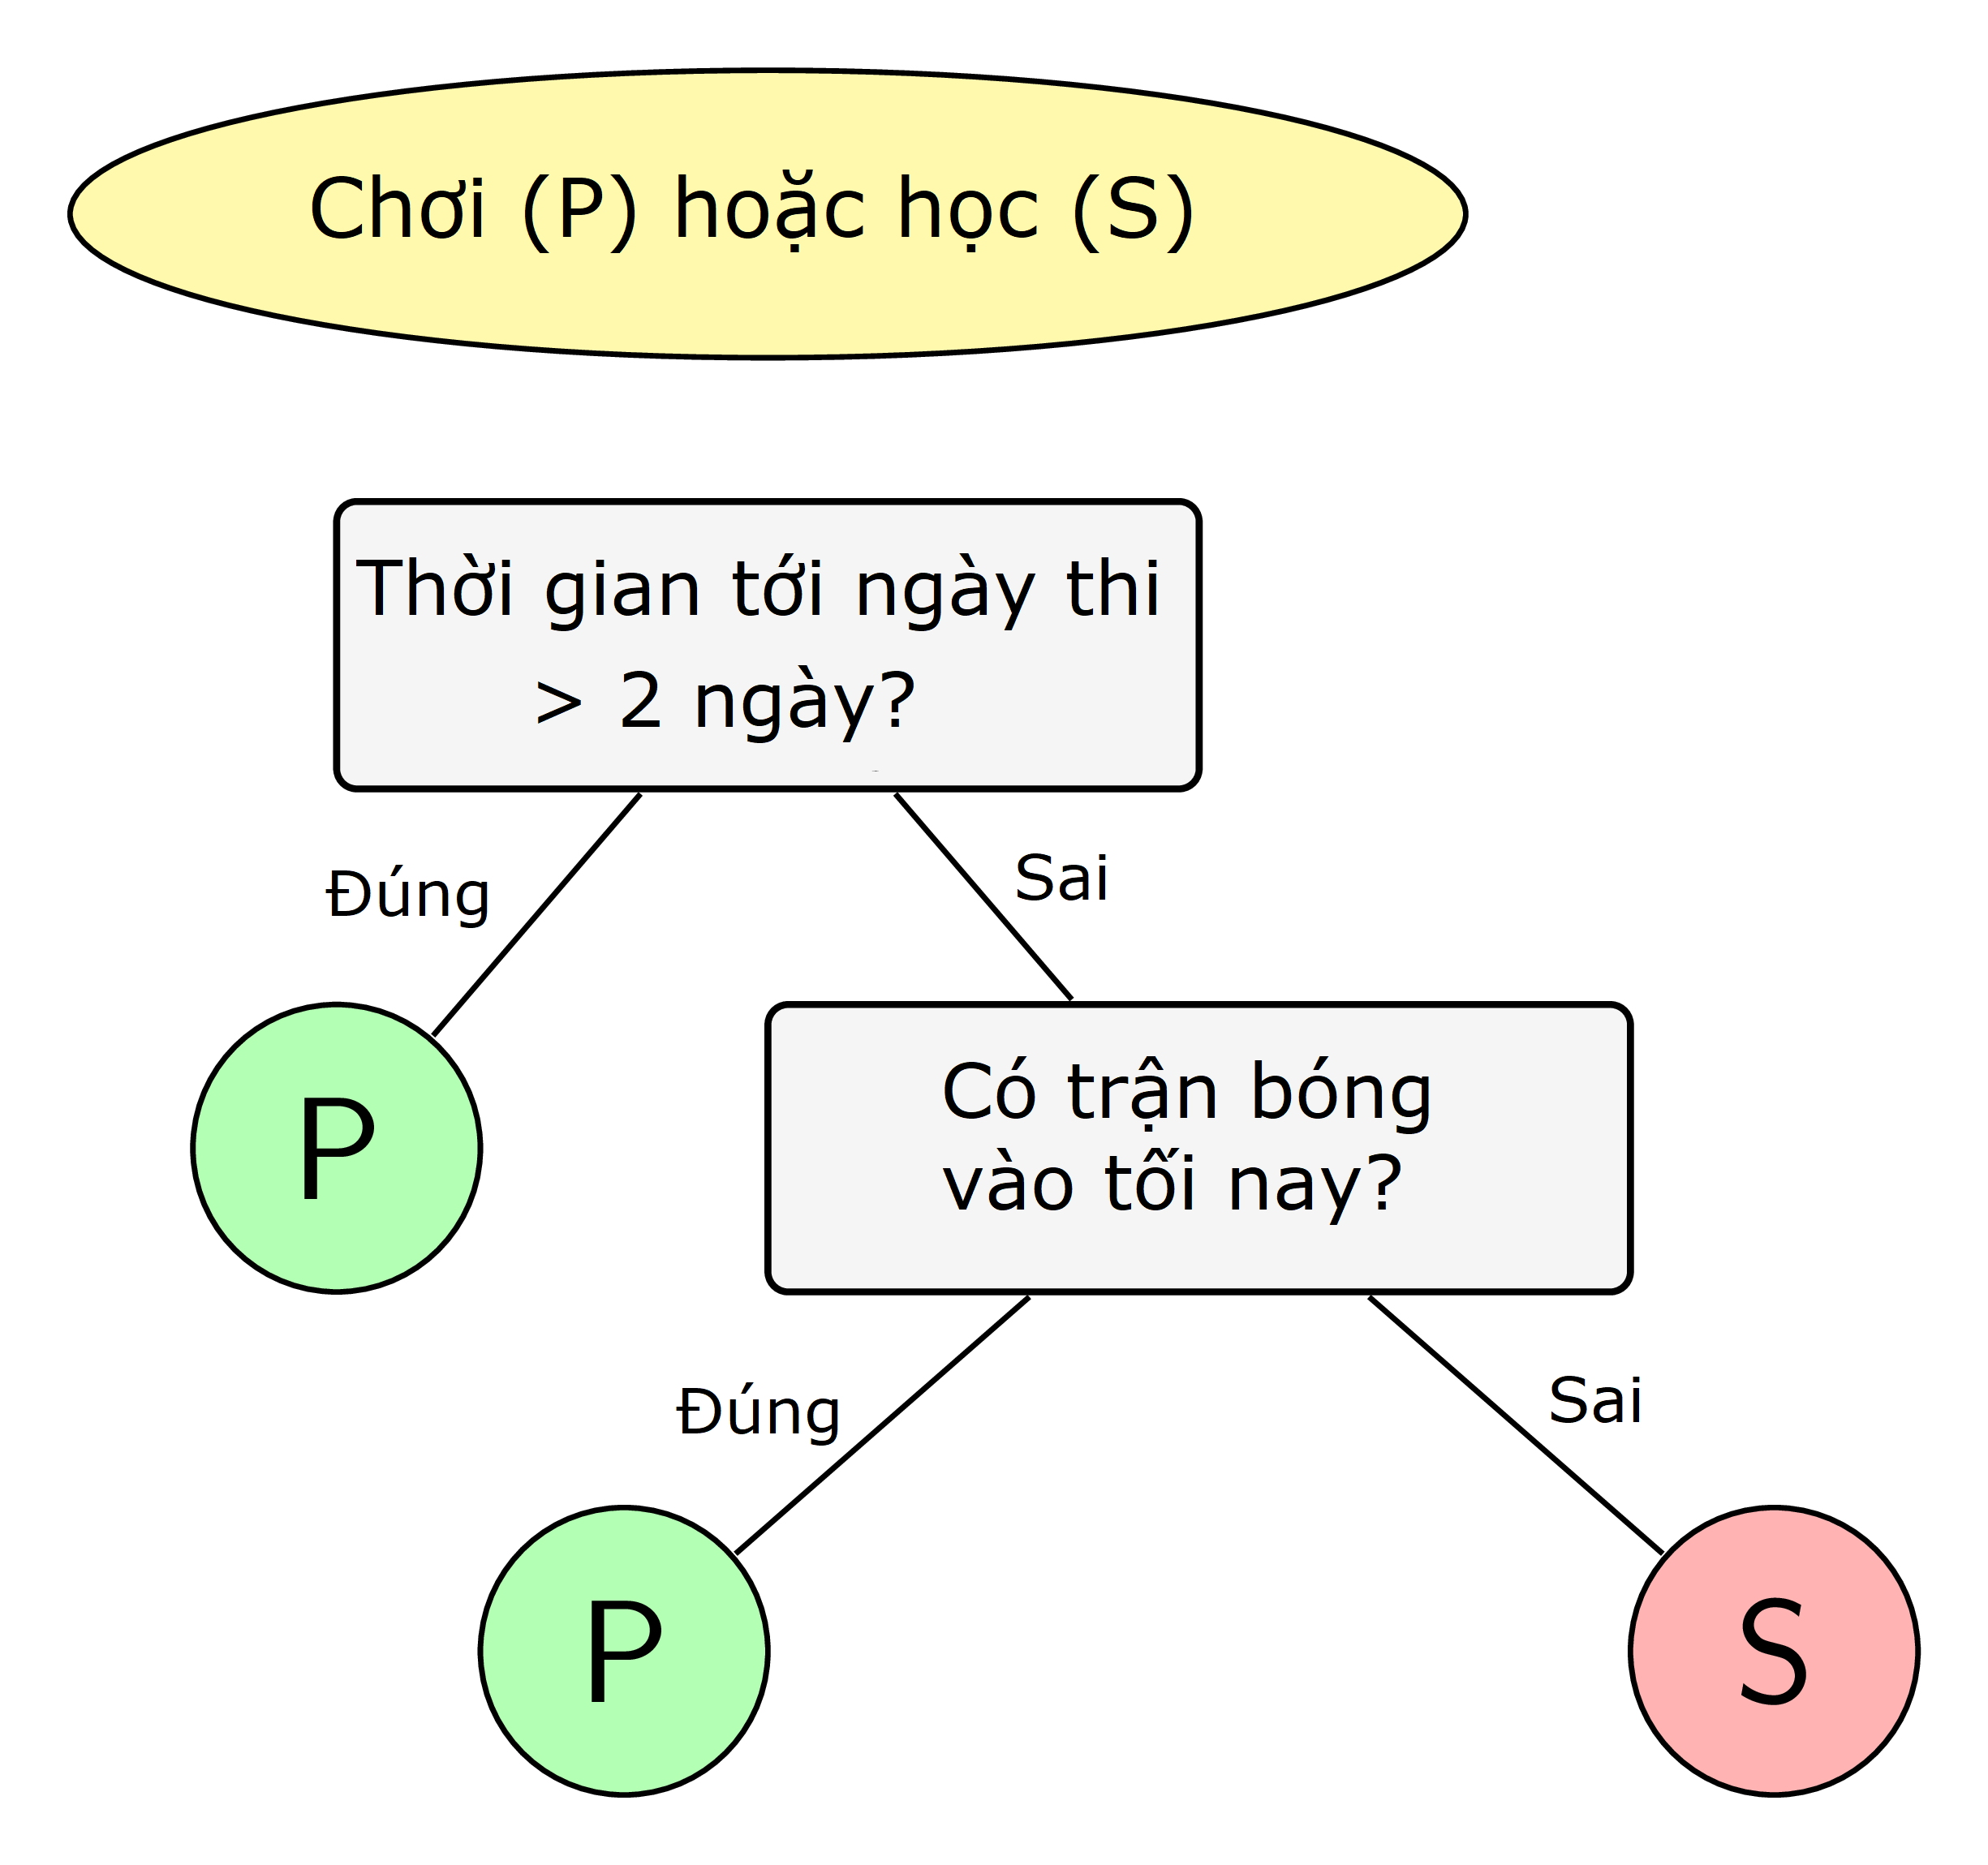
\includegraphics[scale=0.1]{dt_ex1}
\caption{Một ví dụ về việc đưa ra các quyết định dựa trên câu hỏi}
\label{fig:dt_ex1}
\end{figure}

Hình ellipse nền vàng thể hiện quyết định cần được đưa ra. Quyết định này phụ thuộc vào các câu trả lời của các câu hỏi trong các ô hình chữ nhật màu xám. Dựa trên các câu trả lời, quyết định cuối cùng được cho trong các hình tròn màu lục (chơi) và đỏ (học).

Việc quan sát, suy nghĩ và ra các quyết định của con người thường được bắt đầu từ các câu hỏi. Machine learning cũng có một mô hình ra quyết định dựa trên các câu hỏi. Mô hình này có tên là \textit{cây quyết định (decision tree)}.

Trong \textbf{decision tree}, các ô màu xám, lục, đỏ trên hình \ref{fig:dt_ex1} được gọi là các node. Các node thể hiện đầu ra (màu lục và đỏ) được gọi là \textit{node lá} (\textit{leaf node} hoặc \textit{terminal node}). Các node thể hiện câu hỏi là các \textit{non-leaf node}. Non-leaf node trên cùng (câu hỏi đầu tiên) được gọi là node gốc (\textit{root node}). Các non-leaf node thường có hai hoặc nhiều node con (\textit{child node}). Các child node này có thể là một leaf node hoặc một non-leaf node khác. Các child node có cùng bố mẹ được gọi là \textit{sibling node}. Nếu tất cả các non-leaf node chỉ có hai child node, ta nói rằng đó là một \textit{binary decision tree} (cây quyết định nhị phân). Các câu hỏi trong binary decision tree đều có thể đưa được về dạng câu hỏi đúng hay sai. Các decision tree mà một leaf node có nhiều child node cũng có thể được đưa về dạng một binary decision tree. Điều này có thể đạt được vì hầu hết các câu hỏi đều có thể được đưa về dạng câu hỏi đúng sai.

Ví dụ, ta có thể xác định được tuổi của một người dựa trên nhiều câu hỏi đúng sai dạng: tuổi của bạn lớn hơn $x$ đúng không? (Đây chính là thuật toán \textit{tìm kiếm nhị phân – binary search}.)

Decision tree là một mô hình \textit{supervised learning}, có thể được áp dụng vào cả hai bài toán \textit{classification và regression}. Việc xây dựng một decision tree trên dữ liệu huấn luyện cho trước là việc đi xác định các câu hỏi và thứ tự của chúng. Một điểm đáng lưu ý của decision tree là nó có thể làm việc với các đặc trưng (trong các tài liệu về decision tree, các đặc trưng thường được gọi là thuộc tính – \textit{attribute}) dạng \textit{categorical}, thường là rời rạc và không có thứ tự. Ví dụ, mưa, nắng hay xanh, đỏ, v.v. Decision tree cũng làm việc với dữ liệu có vector đặc trưng bao gồm cả thuộc tính dạng categorical và liên tục (numeric). Một điểm đáng lưu ý nữa là decision tree ít yêu cầu việc chuẩn hoá dữ liệu.

\subsection{Phân loại}
Có 3 loại decision trees phổ biến sau:

\begin{itemize}
\item \textbf{ID3 (Iterative Dichotomiser 3)} - Tạo cây nhiều chiều, tìm cho mỗi node một đặt tính phân loại sao cho đặt tính này có giá trị ``information gain'' lớn nhất. Cây được phát triển tới mức tối đa kích thước. Sau đó áp dụng phương thức cắt tỉa cành để xử lý những dữ liệu chưa nhìn thấy.
\item \textbf{C4.5} - Kế thừa từ  ID3 nhưng loại bỏ hạn chế về việc chỉ sử dụng đặc tính có giá trị phân loại bằng cách tự động định nghĩa một thuộc tính rời rạc. Dùng để phân chia những thuộc tính liên tục thành những tập rời rạc.
\item \textbf{CART (Classification and Regression Trees)} - Tương tự như C4.5, nhưng nó hỗ trợ thêm đối tượng dự đoán là giá trị số (\textit{Regression}). Cấu trúc CART dạng cây nhị phân, mỗi node sử dụng một ngưỡng để đạt được ``information gian'' lớn nhất.
\end{itemize}

Hình \ref{fig:decision_tree_type_comparison} so sánh giữa các loại thuật toán decision tree.

\begin{figure}[ht!]
\centering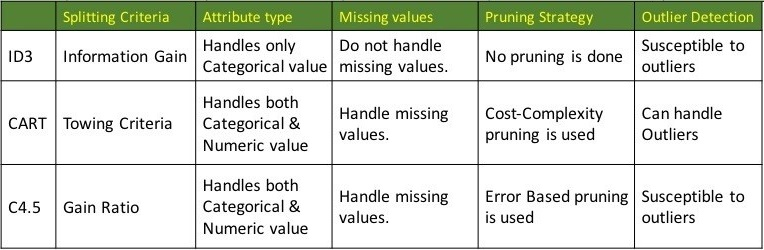
\includegraphics[scale=0.75]{comparison-decision-trees}
\caption{So sánh các thuật toán Decision Trees}
\label{fig:decision_tree_type_comparison}
\end{figure}

\subsection{Ưu và nhược điểm của thuật toán}
Tùy vào loại Decision tree sử dụng mà ta có ưu nhược điểm riêng. Nhưng nhìn chung thuật toán có những ưu nhược điểm chung như sau:
\subsubsection*{Về ưu điểm}
\begin{itemize}
\item Decision tree thường mô phỏng cách suy nghĩ con người. Vì vậy nó đơn giản để hiểu và diễn giải dữ liệu.
\item Giúp ta nhìn thấy được sự logic của dữ liệu ( không như thuật toán phần laoij SVM, KNN …)
\item Có khả năng chọn được những features tốt nhất.
\item Phân loại dữ liệu không cần tính toán phức tạp.
\item Giải quyết vấn đề nhiễu và thiếu dữ liệu.
\item Có khả năng xử lý dữ liệu có biến liên tục và rời rạc.
\end{itemize}

\subsubsection*{Về nhược điểm}
\begin{itemize}
\item Tỉ lệ tính toán tăng theo hàm số mũ còn vấn đề ngày càng lớn hơn.
\item Dễ bị vấn đề overfitting và high bias khi tập dữ liệu huấn luyện nhỏ.
\end{itemize}

Trong bài báo cáo này chúng tôi sử dụng loại \textbf{CART}. Do tính đơn giản, dể tiếp cận của nó, cũng như những giá trị feature mà ta sử dụng là kiểu dữ liệu biến liên tục không phải phân loại nên không dùng \textbf{ID3} được. Và đây là loại decision tree được thư viện \textit{scikit-learn} chọn sử dụng.
\subsection{Làm sạch dữ liệu}

\subsection{Quá trình xây dựng cây}

\section[Một số lỗ hổng web]{Một số lỗ hổng tấn công web phổ biến}
\subsection{SQL Injection}

\subsection{Cross-Site Scripting (XSS)}

\end{document}